\documentclass[]{report}

\usepackage[margin=1.1in]{geometry}
\usepackage{graphicx}

\usepackage{url}
\makeatletter
\g@addto@macro{\UrlBreaks}{\UrlOrds}
\makeatother


\usepackage{float}
\usepackage[utf8]{inputenc}    % For the umlaut in my name...

\usepackage{listings}
\usepackage{hyperref}
\usepackage{xcolor}
\hypersetup {
  colorlinks,
  linkcolor={blue!50!black},
  urlcolor={blue}
}

\definecolor{mygreen}{rgb}{0,0.6,0}
\definecolor{mygray}{rgb}{0.5,0.5,0.5}
\definecolor{mymauve}{rgb}{0.58,0,0.82}

\lstset{ %
	backgroundcolor=\color{white},   % choose the background color; you must add \usepackage{color} or \usepackage{xcolor}; should come as last argument
	basicstyle=\footnotesize,        % the size of the fonts that are used for the code
	breakatwhitespace=false,         % sets if automatic breaks should only happen at whitespace
	breaklines=true,                 % sets automatic line breaking
	captionpos=b,                    % sets the caption-position to bottom
	commentstyle=\color{mygray},    % comment style
	deletekeywords={...},            % if you want to delete keywords from the given language
	escapeinside={\%*}{*)},          % if you want to add LaTeX within your code
	extendedchars=true,              % lets you use non-ASCII characters; for 8-bits encodings only, does not work with UTF-8
	frame=single,	                   % adds a frame around the code
	keepspaces=true,                 % keeps spaces in text, useful for keeping indentation of code (possibly needs columns=flexible)
	keywordstyle=\color{orange},       % keyword style
	language=C,                 % the language of the code
	morekeywords={*,...},            % if you want to add more keywords to the set
	numbers=left,                    % where to put the line-numbers; possible values are (none, left, right)
	numbersep=5pt,                   % how far the line-numbers are from the code
	numberstyle=\tiny\color{mygreen}, % the style that is used for the line-numbers
	rulecolor=\color{black},         % if not set, the frame-color may be changed on line-breaks within not-black text (e.g. comments (green here))
	showspaces=false,                % show spaces everywhere adding particular underscores; it overrides 'showstringspaces'
	showstringspaces=false,          % underline spaces within strings only
	showtabs=false,                  % show tabs within strings adding particular underscores
	stepnumber=1,                    % the step between two line-numbers. If it's 1, each line will be numbered
	stringstyle=\color{mymauve},     % string literal style
	tabsize=2,	                   % sets default tabsize to 2 spaces
	title=\lstname                   % show the filename of files included with \lstinputlisting; also try caption instead of title
}

\lstset{literate=
	{á}{{\'a}}1 {é}{{\'e}}1 {í}{{\'i}}1 {ó}{{\'o}}1 {ú}{{\'u}}1
	{Á}{{\'A}}1 {É}{{\'E}}1 {Í}{{\'I}}1 {Ó}{{\'O}}1 {Ú}{{\'U}}1
	{à}{{\`a}}1 {è}{{\`e}}1 {ì}{{\`i}}1 {ò}{{\`o}}1 {ù}{{\`u}}1
	{À}{{\`A}}1 {È}{{\'E}}1 {Ì}{{\`I}}1 {Ò}{{\`O}}1 {Ù}{{\`U}}1
	{ä}{{\"a}}1 {ë}{{\"e}}1 {ï}{{\"i}}1 {ö}{{\"o}}1 {ü}{{\"u}}1
	{Ä}{{\"A}}1 {Ë}{{\"E}}1 {Ï}{{\"I}}1 {Ö}{{\"O}}1 {Ü}{{\"U}}1
	{â}{{\^a}}1 {ê}{{\^e}}1 {î}{{\^i}}1 {ô}{{\^o}}1 {û}{{\^u}}1
	{Â}{{\^A}}1 {Ê}{{\^E}}1 {Î}{{\^I}}1 {Ô}{{\^O}}1 {Û}{{\^U}}1
	{œ}{{\oe}}1 {Œ}{{\OE}}1 {æ}{{\ae}}1 {Æ}{{\AE}}1 {ß}{{\ss}}1
	{ű}{{\H{u}}}1 {Ű}{{\H{U}}}1 {ő}{{\H{o}}}1 {Ő}{{\H{O}}}1
	{ç}{{\c c}}1 {Ç}{{\c C}}1 {ø}{{\o}}1 {å}{{\r a}}1 {Å}{{\r A}}1
	{€}{{\euro}}1 {£}{{\pounds}}1 {«}{{\guillemotleft}}1
	{»}{{\guillemotright}}1 {ñ}{{\~n}}1 {Ñ}{{\~N}}1 {¿}{{?`}}1
}

% call as such : \lstinputlisting[language=C]{interface.h}

\providecommand{\tightlist}{%
	\setlength{\itemsep}{0pt}\setlength{\parskip}{0pt}}

%\title{Audio processing on the BeagleBone Black's Programmable Real-time Unit}
%\author{Loïc Droz}
%\date{Bachelor Semester Project - Fall 2017}


%\usepackage{titling}
%\pretitle{%
%	\begin{center}
%		\LARGE
%		
\includegraphics[width=0.5\linewidth]{Pictures/epfl}\\
%		[\bigskipamount]
%	}
%\posttitle{
%	\end{center}}

\begin{document}

%\maketitle

%\begin{titlepage}
%	\centering
%	\vfill
%	{\bfseries\Large
%		Audio processing on the BeagleBone Black's Programmable Real-time Unit\\
%		Bachelor Semester Project - Fall 2017 \\
%		\vskip2cm
%		Loïc Droz\\
%	}    
%	\vfill
%	
\includegraphics[width=0.5\linewidth]{Pictures/epfl}
%	\vfill
%	\vfill
%\end{titlepage}


\begin{titlepage}
	\centering
	\vspace*{50px}
	\vfill
	{
		\textbf{\LARGE Audio Processing on the BeagleBone Black's Programmable Real-time Unit}\\
		\vskip0.5cm
		{\LARGE Bachelor Semester Project - Fall 2017} \\
		\vskip2cm
		{\Large Loïc Droz}\\
	}    
	\vfill
	\vskip5cm
	
\includegraphics[width=0.5\linewidth]{Pictures/epfl}
%	\vfill
%	\vfill
\end{titlepage}


\tableofcontents


\hypertarget{introduction-motivation}{%
\chapter{Introduction / Motivation}\label{introduction-motivation}}

The goal of this project is to implement audio processing using one of the BeagleBone Black's PRU microprocessors along with a C API built around it to make it easily usable as a simple C library. The input signals come from 6 Knowles SPM1437HM4H-B microphones connected to the board, each with a 1-bit wide signal (Pulse Density Modulation, see Section~\ref{audio-processing}).

The audio processing code currently handles the six microphones at a fixed output sample rate, using one of the 2 PRUs present on the board. For now, the API is very simple. It allows the user to read the processed data from the PRU to a user-supplied buffer, specify the quantity of data needed and the number of channels to extract from it. It also allows the user to pause and resume the recording of the data on the API side in order to prevent overflows in case the user wants to momentarily stop reading data.

Running the core audio processing code on the PRU instead of the main ARM CPU allows for lower latency due to the PRU's predictable timing and it not being subject to OS scheduling like a typical Linux process running on the ARM CPU would be. Offloading the ARM CPU from such an intensive task also prevents our library from having a significant impact on the global performance of the host when it is used.

The code and documentation can be found at the link below:
\begin{center}
	\url{https://github.com/Scrashdown/PRU-Audio-Processing}
\end{center}

%\hypertarget{theory}{%
%	\chapter{Theory}\label{theory}}
	\chapter{Background Knowledge}
	\label{theory}

\hypertarget{pru-pruss}{%
\section{PRU / PRUSS}\label{pru-pruss}}

The PRUSS is a module of the ARM CPU used on the BeagleBone Black. It stands for PRU SubSystem, where PRU stands for Programmable Real-time Unit. The PRUSS contains 2 PRUs which are essentially very small and simple 32-bit microprocessors running at 200 MHz and use a custom instruction set. Each PRU has a constant 200 MHz clock rate, 8 kB of instruction memory, 8 kB of data memory, along with 12 kB of data memory shared between the 2 PRUs. They can be programmed either in assembly using the \texttt{pasm} assembler or in C using the \texttt{clpru} and \texttt{lnkpru} tools.

Each PRU has 32, 32-bit registers, where R30 is used for interacting with the PRU's output pins and R31 is used for reading inputs from these pins and triggering interrupts by writing to it. Both PRUs also share 3 registers banks, also called \emph{scratchpads}, which each contain 30 additional registers. Registers can be transferred in and out between these banks and each PRU in one cycle by using specialized assembly instructions (\texttt{XIN} / \texttt{XOUT} / \texttt{XCHG}, commonly called \texttt{XFR} instructions in the PRU Reference Manual). Furthermore, one PRU can also access the registers of the other PRU using the same assembly instructions.

The PRUs are designed to be as time-deterministic as possible. That is, pretty much all instructions will execute in a constant number of cycles (usually 1, therefore in 5 ns at the 200 MHz clock rate) except for the memory instructions which may vary in execution time.

The PRUSS also contains an interrupt controller which allows the PRU to send and receive interrupts to and from the ARM CPU. It can be configured either from the PRUs themselves by changing the values of the configuration registers, or from the ARM CPU using the \texttt{prussdrv} library along with the \texttt{uio\_pruss} driver (more information on that in Section~\ref{configure-uio-pruss-and-free-the-gpio-pins-for-the-pru}).

Using the PRUSS requires a driver. Currently, there are 2 choices available : \texttt{uio\_pruss} (along with the \texttt{prussdrv} library) and the newer \texttt{pru\_rproc}. \texttt{uio\_pruss} provides a lower level interface than \texttt{pru\_rproc}. \texttt{pru\_rproc} provides a C library for message passing between the PRU and the ARM CPU which makes programming simpler than with \texttt{uio\_pruss}. However, the current lack of examples online for using \texttt{pru\_rproc}, along with performance issues encountered using it for this project, made us choose \texttt{uio\_pruss} instead.

That said, it seems \texttt{uio\_pruss} is currently being phased out of support by Texas Instruments in favor of \texttt{pru\_rproc}. It may be feasible in the future to convert the code to use \texttt{pru\_rproc}. However, as we are going to see further in the report, the timing requirements in the PRU processing code are very tight, even using assembly. Whether it would be possible to meet them using C and \texttt{pru\_rproc} has yet to be investigated.

\hypertarget{audio-processing}{%
\section{Audio Processing}\label{audio-processing}}

For this project, we are using microphones with a 1-bit wide output at a very high sample rate ($ > $~1~MHz). This type of signal is known as a PDM (Pulse Density Modulation) signal and needs to be converted to a lower-rate PCM (Pulse-Code Modulation) signal, which is much more commonly used for processing and storing audio data.

\begin{figure}[H]
\centering
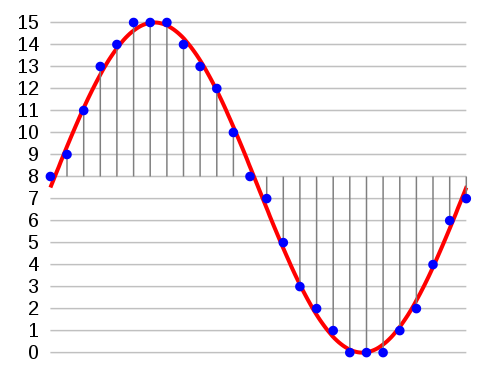
\includegraphics[width=0.7\linewidth]{Pictures/PCM.png}
\caption{Illustration of a PCM signal (CC BY-SA 3.0, \url{https://commons.wikimedia.org/w/index.php?curid=635225)}}
\end{figure}

\begin{figure}[H]
\centering
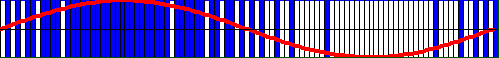
\includegraphics[width=1.0\linewidth]{Pictures/PDM.png}
\caption{Illustration of a PDM}
\end{figure}

In a PCM signal, each value represents its amplitude on a fixed scale at a fixed time. However, in a PDM signal, its amplitude at a given time is represented by the density of 1's relative to 0's at a given time. Converting a PDM signal to a PCM signal therefore requires using some form of a moving-average filter.

\hypertarget{cic-filter}{%
\subsection{CIC Filter}\label{cic-filter}}

Because we wanted to run this filter on the PRU with rather tight timing constraints, we chose to implement a Cascaded Integrator-Comb (CIC) filter. There are two general types of CIC filters: the decimation filters, which is the type we are using in this project, and the interpolation filters. From now on we will refer to CIC decimator filters simply as CIC filters.

The CIC filter is essentially an efficient implementation of a moving-average filter by using only additions and subtractions and has a finite-length impulse response (FIR). Although the PRU is capable of performing unsigned integer multiplications (required by other types of FIR filters) by using its Multiply and Accumulate Unit, they take several more cycles to execute than the one-cycle instructions used for regular additions and subtractions. Since our goal is to handle several channels at once with very tight timing constraints, computational savings really matter.

A CIC filter also has a drawback however. Its frequency response is far from the ideal flat response with a sharp cutoff we would like to have. To get a sharper cutoff, it is necessary to cascade another filter, commonly called a \emph{compensation} filter, to the CIC output. That said, since a CIC filter's output is usually at a much lower rate (64 kHz for now) than its input ($ \approx $1.028 MHz), applying this filter after the CIC filter will require much less computational resources than applying it on the raw, very high rate input signal from the microphones.

In general, CIC filters are well suited as an efficient first filtering step, which efficiently downsamples the signal and gets rid of some of the higher frequencies. The reduced sample rate of the output reduces the computational power needed for additional FIR compensation filters, and therefore compensates their higher complexity.

\begin{figure}
\centering
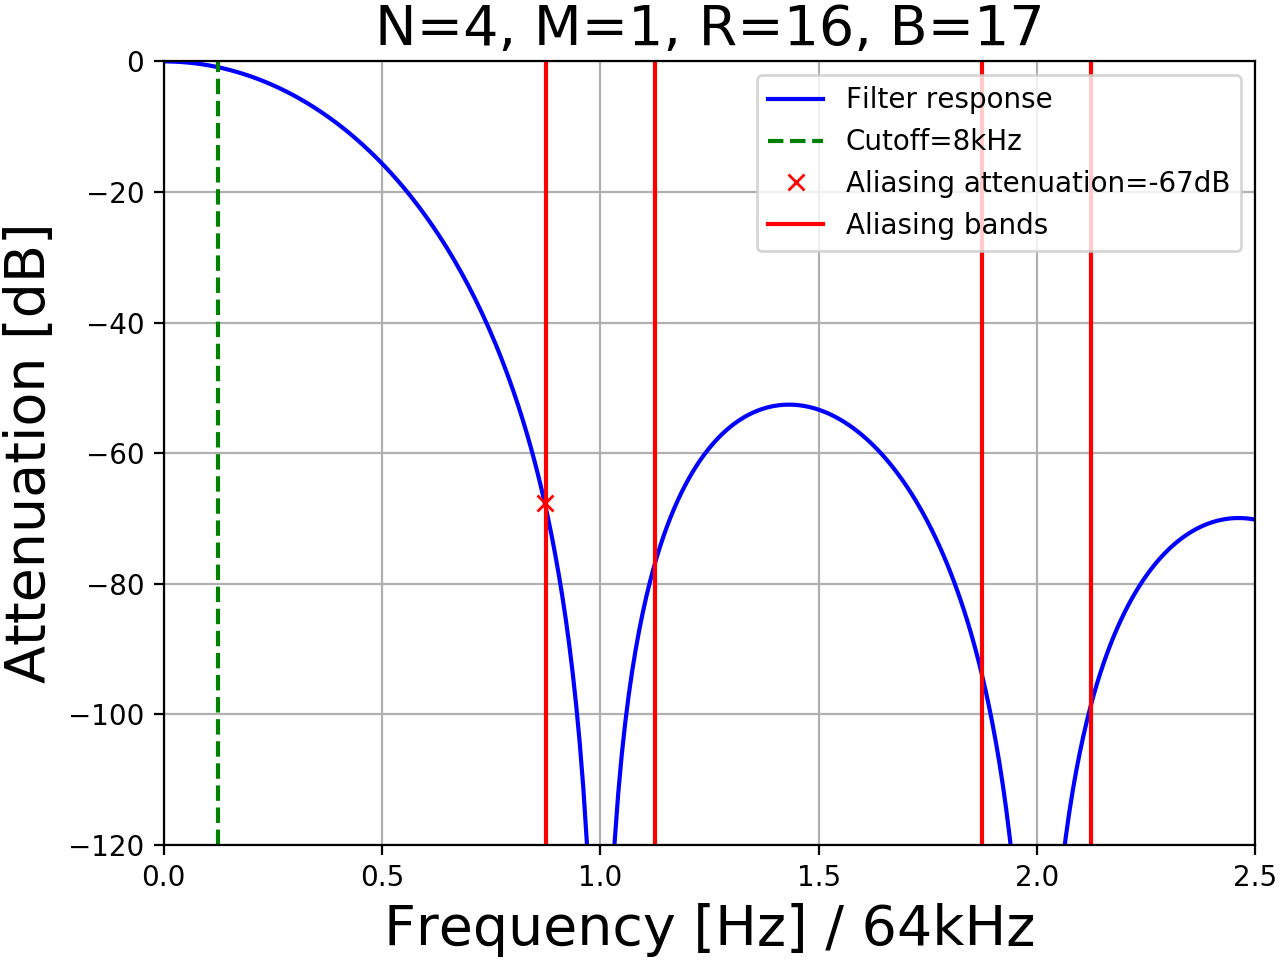
\includegraphics[width=0.9\linewidth]{Pictures/CIC_power_resp.png}
\caption{Example power response of the filter}
\end{figure}

Now let's dive into more detail about the CIC filter. The filter has 3 parameters : N, M, and R. It is made of N cascaded integrator stages, followed by a decimator of rate R, and then N cascaded comb stages, where M is the delay of the samples in the comb stages. It takes a PDM signal as input and outputs a PCM signal. If the input sample rate is \texttt{f\_s}, the output sample rate will be \texttt{f\_s / R}. A CIC interpolation filter is very similar, except the comb stages come first, followed by an interpolator of rate R, and finally the integrators.

\begin{figure}[H]
\centering
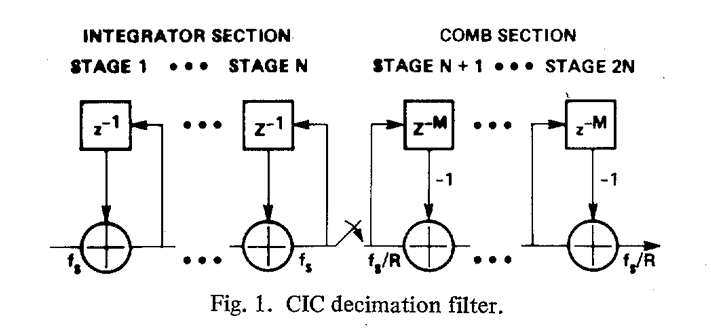
\includegraphics[width=0.9\linewidth]{Pictures/CIC_structure.png}
\caption{Structure of a CIC decimation filter}
\end{figure}

The filter's resource usage depends on its parameters, the platform on which it is implemented and how it is implemented. More detailed explanation will follow in the implementation section of this report - Section~\ref{implementation}. However, by considering only the theoretical structure of the filter, we can already deduce some general rules :

\begin{itemize}
\tightlist
\item
  Memory usage is approximately proportional to N and M : The filter has N integrator stages and N comb stages of which we need to store the values, therefore memory usage is approximately proportional to N. Also, since M is the delay of the samples in the comb stages, for each comb stage it is necessary to store the previous M samples, therefore memory usage is approximately proportional to M.
\item
  Computational resource usage is inversely correlated to R : Since the comb stages are preceded by a decimator of rate R, the comb stages need to be updated R times less often than the integrator stages. Therefore, as R increases, less computational power is required by the comb stages. However, the reduction cannot be arbitrarily high, because the integrator stages always need to be updated at the very high input sample rate, independently of R. The processing power needed for these stages, and any other overhead added by the implementation, constitute therefore a lower-bound of the total processing power required to run the filter.
\end{itemize}

Finally, it is important to note that overflows will occur in the integrator stages. However, the output of the filter will still be correct if each stage follows modular arithmetic rules (PRU registers do, since they can overflow and loop back to zero) and if each stage has a bit width large enough that it can support the maximum possible value at the output of the filter. To ensure the second condition is met, the following formula is used to calculate the required bit width for each stage of the filter (described in Hogenhauer's paper) :

\begin{equation}
\label{eq:bout}
B_{out} = \lceil Nlog_2(RM) + B_{in} \rceil
\end{equation}

\noindent where \(B_{in}\) is the bit width of the filter's input (in our case 1
bit), M, N and R are the filter's parameters, and \(B_{out}\) is the
required bit width for all stages of the filter.

\hypertarget{implementation}{%
\chapter{Implementation}\label{implementation}}

\hypertarget{getting-started}{%
\section{Getting Started}\label{getting-started}}

First of all, make sure you have the required hardware: the BeagleBone
Black, an SD card, and the Kurodako Board. Flash the board with the
latest ``IoT" Debian image following these instructions\footnote{\url{https://beagleboard.org/getting-started}}.

\begin{figure}[H]
\centering
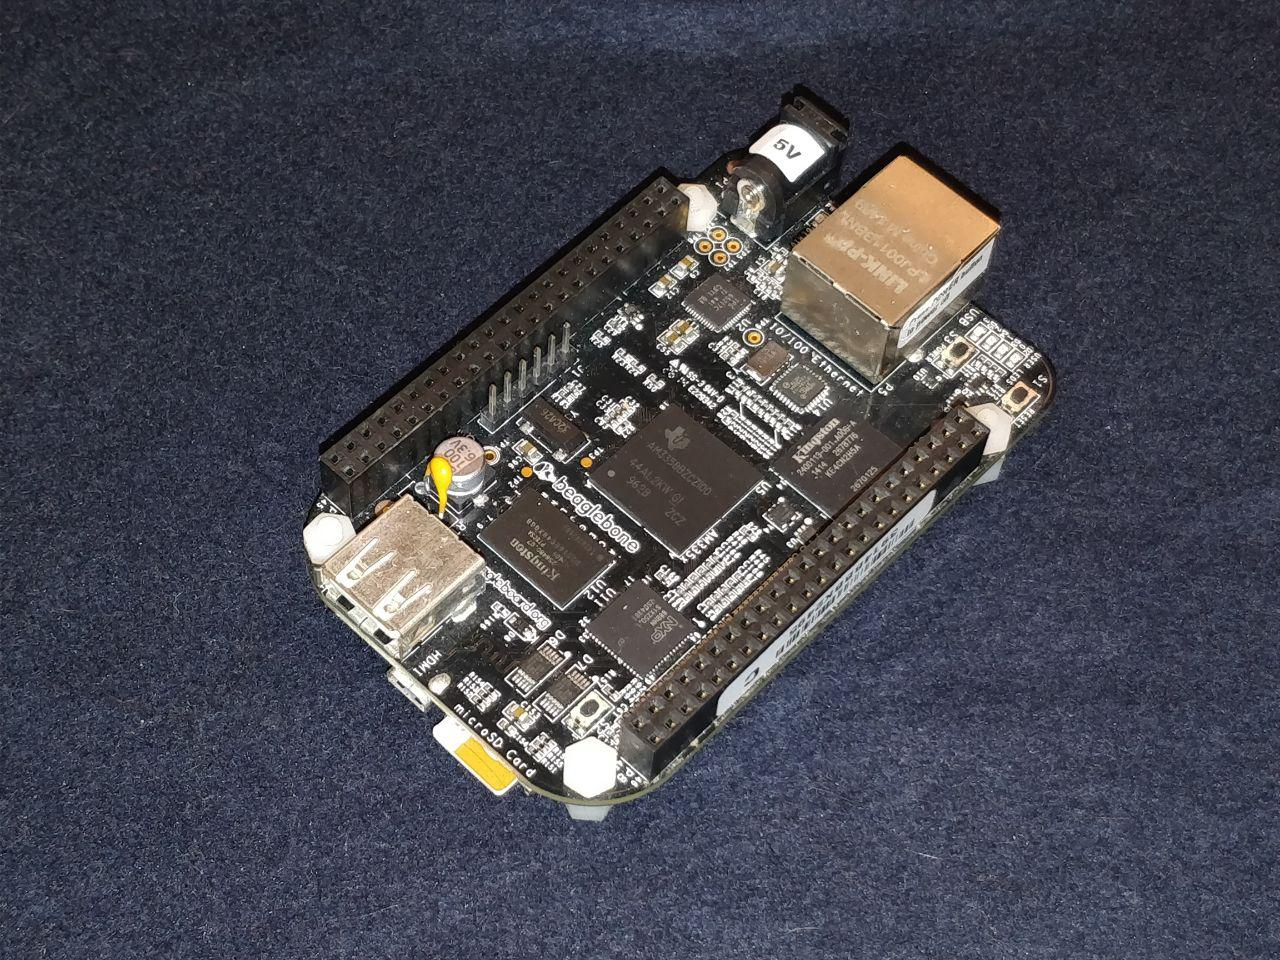
\includegraphics[width=0.9\linewidth]{Pictures/BBB.jpg}
\caption{The BeagleBone Black, with an SD card}
\end{figure}

\begin{figure}[H]
\centering
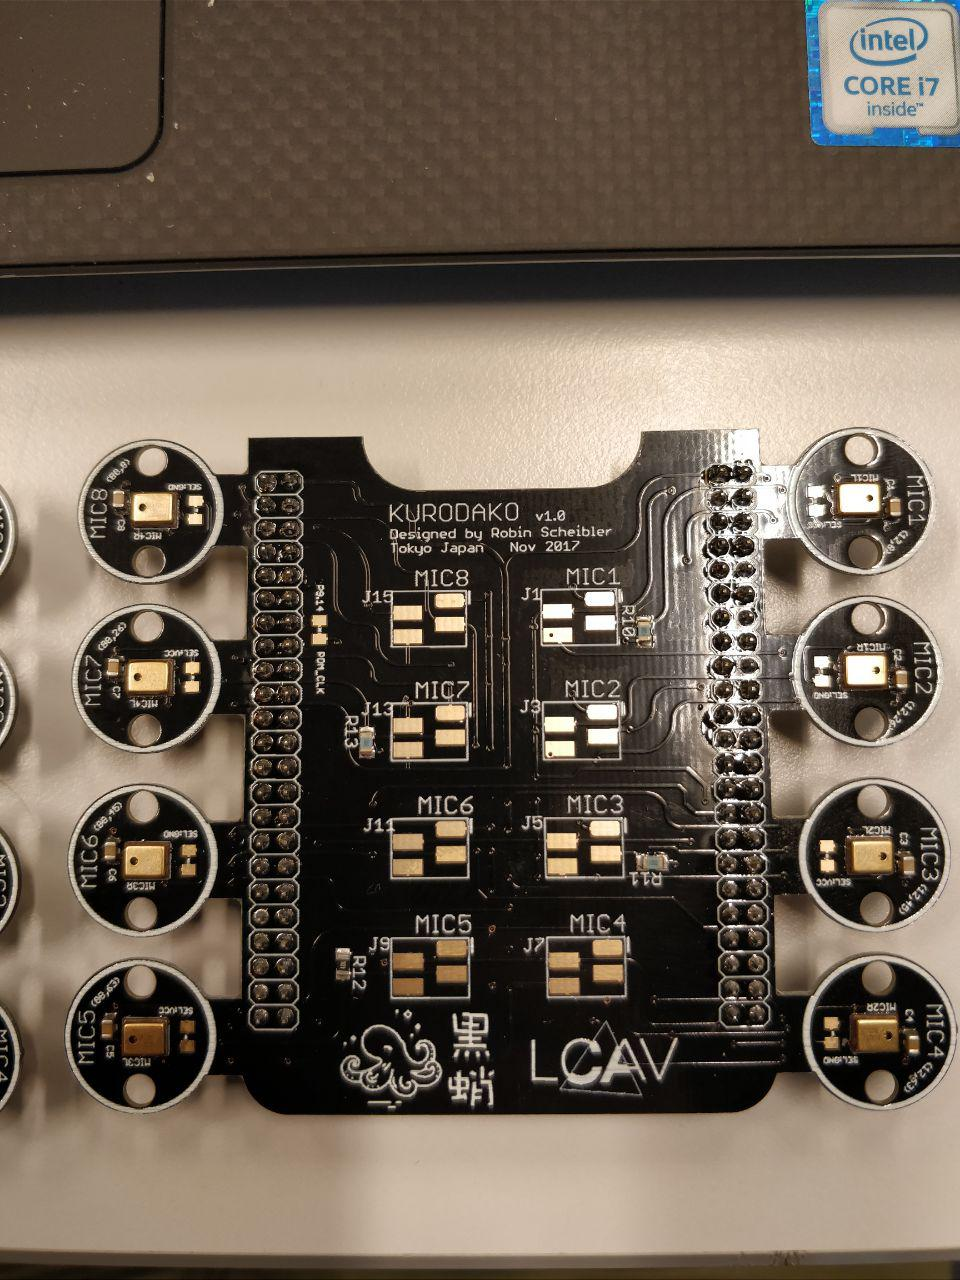
\includegraphics[width=0.4\linewidth]{Pictures/kurodako.jpg}
\caption{The Kurodako Board, although the program only supports 6
channels for now, it has 8 mics.}
\end{figure}

\begin{figure}
\centering
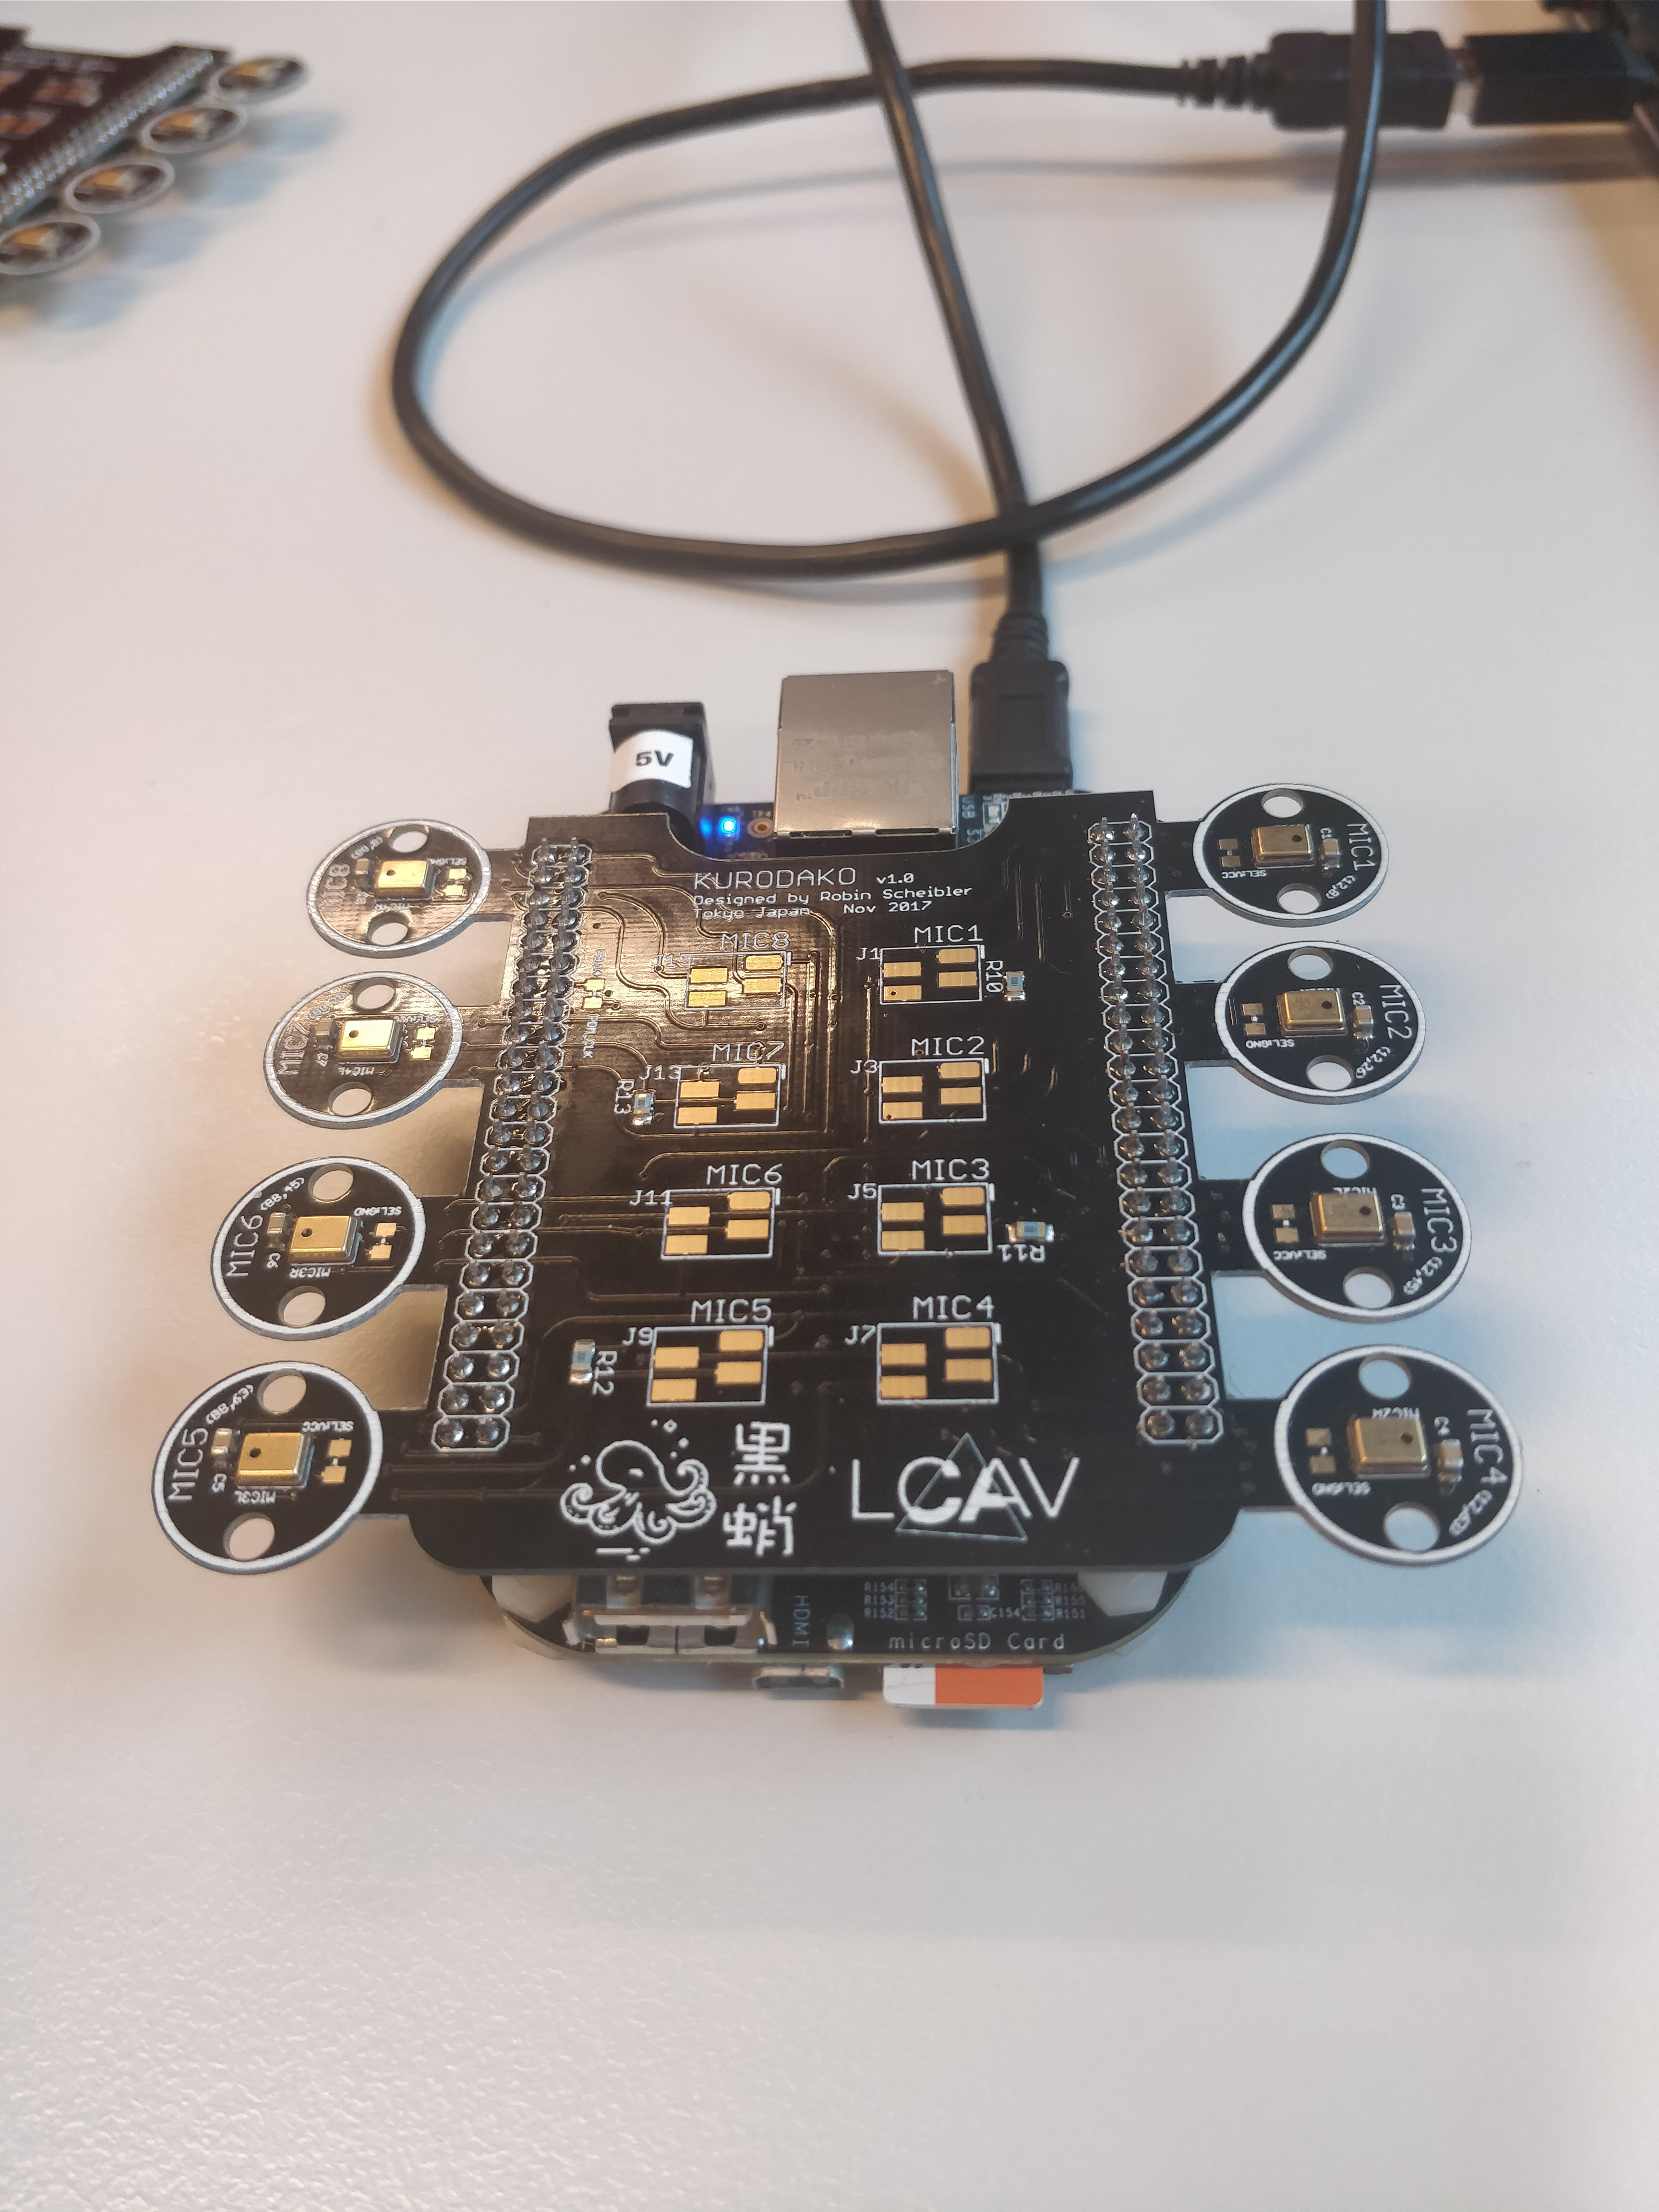
\includegraphics[width=0.4\linewidth]{Pictures/BBBkurodako.jpg}
\caption{The BBB with the Kurodako Board, ready to be used!}
\end{figure}

%\hypertarget{configure-uio\_pruss-and-free-the-gpio-pins-for-the-pru}{%
%\subsection{\texorpdfstring{Configure \texttt{uio\_pruss} and free
%the BBB GPIO pins for the
%PRU}{Configure uio\_pruss and free the BBB GPIO pins for the PRU}}\label{configure-uio\_pruss-and-free-the-gpio-pins-for-the-pru}}

\hypertarget{configure-uio-pruss-and-free-the-gpio-pins-for-the-pru}{%
	\subsection{\texorpdfstring{Configure \texttt{uio\_pruss} and free
			the BBB GPIO pins for the
			PRU}{Configure uio\textunderscore pruss and free the BBB GPIO pins for the PRU}}\label{configure-uio-pruss-and-free-the-gpio-pins-for-the-pru}}

\emph{Note: this was tested on this kernel:}
\texttt{Linux beaglebone\ 4.4.91-ti-r133\ \#1\ SMP\ Tue\ Oct\ 10\ 05:18:08\ UTC\ 2017\ armv7l\ GNU/Linux}

In order to run the filter, we need to be able to use the input pins from the PRUs to be able to read data from the microphones.
The PRU's I/O pins can be connected to the BBB's GPIO pins\footnote{Image of the BBB's GPIO pins : \url{http://beagleboard.org/static/images/cape-headers.png}}. However, by default, some BBB
pins cannot be reassigned to anything else. To correct this, we need to
load a \href{https://elinux.org/Capemgr}{cape}\footnote{\url{https://elinux.org/Capemgr}}. To do so, open the
\texttt{/boot/uEnv.txt} file on the board (backup it first!) and do the
following modifications, then reboot :\\

\noindent Add the following line :

\begin{verbatim}
cape_enable=bone_capemgr.enable_partno=cape-universala
\end{verbatim}

\noindent And comment the following line :

\begin{verbatim}
enable_uboot_cape_universal=1
\end{verbatim}

You should now be able to multiplex a pin to the PRUs using the
\texttt{config-pin} command (see these
\href{Documentation/pins.md}{instructions} for more details). We still
have to enable the UIO driver, which is disabled in favor of
\texttt{pru\_rproc} on this kernel. To do so, still in the
\texttt{/boot/uEnv.txt} file, comment the following line :

\begin{verbatim}
uboot_overlay_pru=/lib/firmware/AM335X-PRU-RPROC-4-4-TI-00A0.dtbo
\end{verbatim}

\noindent And uncomment this one :

\begin{verbatim}
uboot_overlay_pru=/lib/firmware/AM335X-PRU-UIO-00A0.dtbo
\end{verbatim}

\noindent Then from the Terminal :

\begin{verbatim}
$ cd /opt/source/dtb-4.4-ti
$ sudo nano src/arm/am335x-boneblack.dts
\end{verbatim}

\noindent Comment this line :

\begin{verbatim}
#include "am33xx-pruss-rproc.dtsi"
\end{verbatim}

\noindent And uncomment this one :

\begin{verbatim}
#include "am33xx-pruss-uio.dtsi"
\end{verbatim}

\noindent Then close nano and run the following commands :

\begin{verbatim}
$ make
$ sudo make install
\end{verbatim}

\noindent This is the final step. Run
\texttt{sudo\ nano\ /etc/modprobe.d/pruss-blacklist.conf} and add the
following lines :

\begin{verbatim}
blacklist pruss
blacklist pruss_intc
blacklist pru-rproc
\end{verbatim}

\noindent Now reboot the board, and you should be able to run commands such as
\texttt{config-pin\ -q\ P8.45} (to query the status of a pin) without trouble.

\hypertarget{install-pruss-driver-library-prussdrv-and-pru-assembler-pasm}{%
\subsection{\texorpdfstring{Install PRUSS Driver Library
(\texttt{prussdrv}) and PRU Assembler
(\texttt{pasm})}{Install PRUSS Driver Library (prussdrv) and PRU Assembler (pasm)}}\label{install-pruss-driver-library-prussdrv-and-pru-assembler-pasm}}

In order to install the PRUSS driver on the host side, first clone this
\href{https://github.com/beagleboard/am335x_pru_package}{repo}\footnote{\url{https://github.com/beagleboard/am335x_pru_package}}. Then
\texttt{cd} into the cloned repository and run the following commands :

\begin{verbatim}
$ make
$ sudo make install
$ sudo ldconfig
\end{verbatim}

If everything went well, the \texttt{prussdrv} library and the
\texttt{pasm} assembler should be installed on your board and ready to
be used.

\hypertarget{plug-the-octopus-board-and-write-some-code}{%
\subsection{Plug the Kurodako board and write some
code!}\label{plug-the-octopus-board-and-write-some-code}}

The code for the CIC filter and the interface can be found in
\texttt{src/6Mic-CIC/}. To write and run some code like the one below,
write it to a file called \texttt{main.c} in \texttt{host/}, then run
\texttt{sh\ deploy.sh}, \texttt{cd\ gen/} and \texttt{./main}.

\lstinputlisting{../src/6Mic-CIC/host/main.c}

\hypertarget{microphones-and-wiring-diagram}{%
\section{Microphones and wiring
diagram}\label{microphones-and-wiring-diagram}}

\begin{figure}[H]
\centering
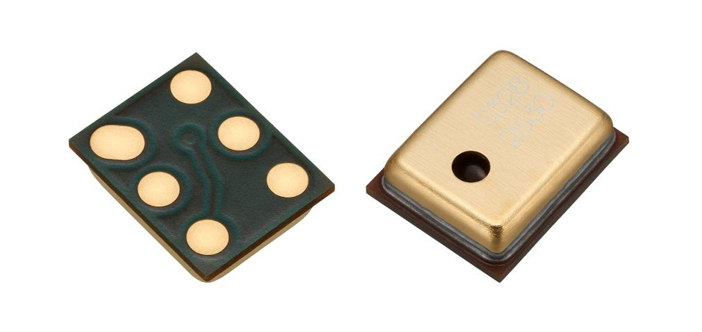
\includegraphics[width=0.6\linewidth]{Pictures/mics.png}
\caption{Knowles SPM1437HM4H-B microphones}
\end{figure}

For this project, we are using the Knowles SPM1437HM4H-B microphones
which output a PDM signal at a very high frequency (\textgreater{} 1
MHz), see the microphone's datasheet\footnote{\url{https://media.digikey.com/pdf/Data\%20Sheets/Knowles\%20Acoustics\%20PDFs/SPM1437HM4H-B.pdf}} for more
details. They have 6 pins :

\begin{itemize}
\tightlist
\item
  2 x \textbf{GROUND} (power) : Ground.
\item
  \textbf{VDD} (power) : VDD.
\item
  \textbf{CLK} (input) : The clock input, must be at a frequency
  \textgreater{} 1 MHz to wake up the microphone. Dictates the
  microphone's sample rate, \texttt{f\_s\ =\ f\_clk}.
\item
  \textbf{DATA} (output) : The microphone's PDM output. Its sample rate
  equals the period of the CLK signal. The DATA signal is ready shortly
  after the rising or falling edge of the CLK. This delay is variable,
  but is between 18 ns and 125 ns. It is designated in the microphone's datasheet
  as \texttt{t\_dv}.
\item
  \textbf{SELECT} (input) : Selects whether data is ready after rising
  or falling edge of CLK, (VDD =\textgreater{} rising, GND
  =\textgreater{} falling).
\end{itemize}

The BeagleBone Black already has pins for GND and VDD, we connect them directly to the corresponding pins on the microphones.

The CLK signal is generated using one of the BeagleBone's internal PWM which is output to one of the board's pins and is configured by a bash script to generate an appropriate CLK period for the microphones. In our implementation, the PRUs also need to be able to poll the state of the CLK signal. In order to achieve this, the PWM (CLK) signal is also connected to some of the BeagleBone's pins, which are multiplexed to the PRU.

The DATA pin of the microphone is then connected to a pin of the board which is multiplexed to the PRU.

\begin{figure}[H]
\centering
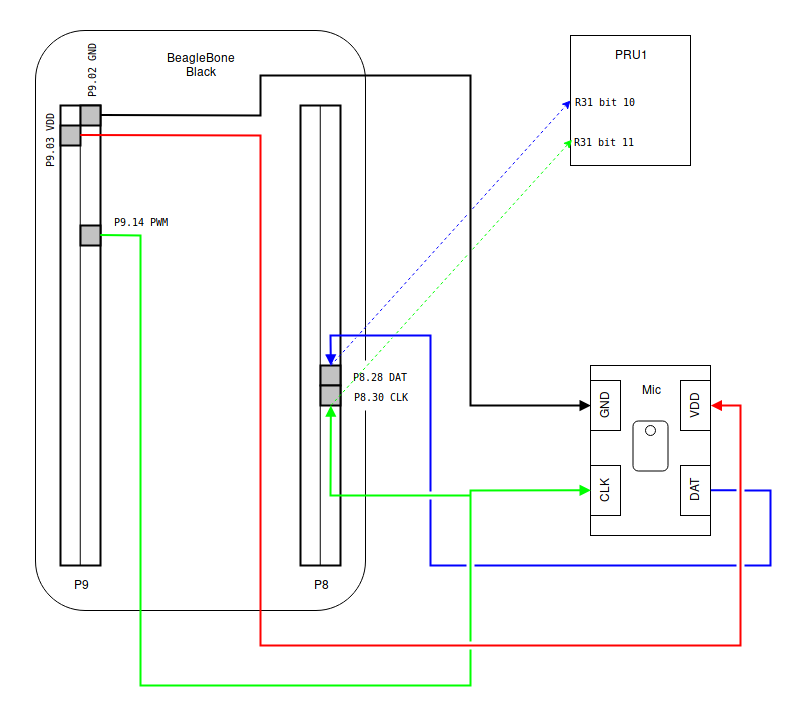
\includegraphics[width=0.6\linewidth]{Pictures/wiring.png}
\caption{Wiring of one microphone to the board}
\end{figure}

Since we are using 6 microphones, we could use 6 pins on the board for the microphone's DATA outputs, however it is possible to connect 2 microphones to a single board pin, thus tying two DATA lines together. To achieve this, we set one of the SELECT lines of the microphones to VDD and the other to GND. By doing this, one of the microphones will have data ready just after the rising edge of the input clock, while the other one will have data ready just after the falling edge. In order to avoid a short circuit between the 2 microphones connected to the same pin, it is necessary to place a resistor between one of the microphones (for example, between all rising edge microphones) and the BeagleBone Black pin. This method has the advantage of using 3 pins on the BBB instead of 6.

Doing this has a drawback however, for each round of processing (processing all the channels) we need to wait for \texttt{t\_dv} twice instead of only once with the `simple' solution using 6 pins. This is because in this case, to retrieve data from all microphones, we have to wait for \texttt{t\_dv} after the rising edge \emph{and} after the falling edge of the clock. According to the microphone's datasheet \footnote{\url{https://media.digikey.com/pdf/Data\%20Sheets/Knowles\%20Acoustics\%20PDFs/SPM1437HM4H-B.pdf}}, \texttt{t\_dv} can go up to 125 ns, which is 25 cycles of the PRU at its 200 MHz clock rate. Although not a huge advantage in performance it is still significant. However, the current Kurodako board uses the 3 pins for 6 microphones, so we have to deal with this drawback.

\begin{figure}[H]
\centering
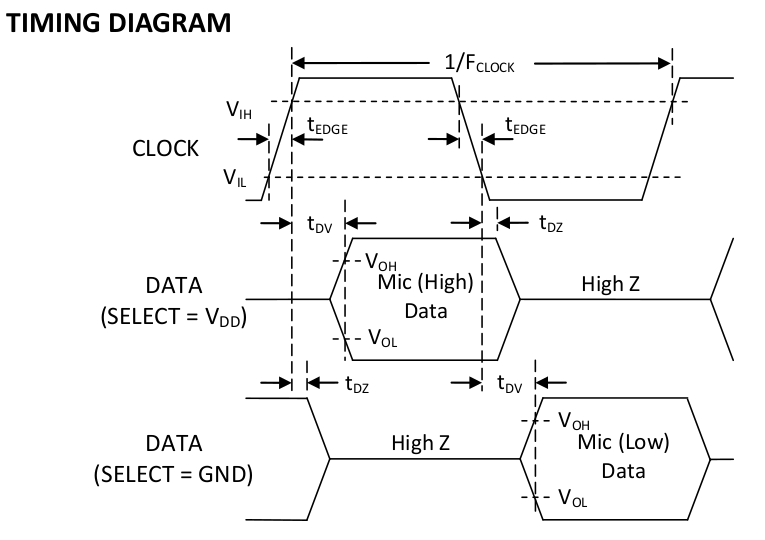
\includegraphics[width=0.6\linewidth]{Pictures/timing_diagram.png}
\caption{Timing diagram of the microphones}
\end{figure}

%\newpage

\hypertarget{overview-of-the-whole-processing-chain}{%
\section{Overview of the whole processing
chain}\label{overview-of-the-whole-processing-chain}}

\begin{figure}[H]
\centering
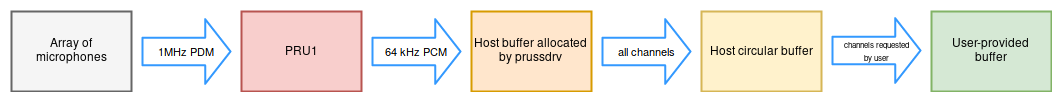
\includegraphics[width=1.0\linewidth]{Pictures/PRU_processing_chain.png}
\caption{Overview of the whole processing chain}
\end{figure}

The complete processing chain is made of several elements :

\begin{itemize}
\tightlist
\item
  \textbf{The array of microphones} : Each microphone generates a 1.028 MHz PDM signal sent to PRU1.
\item
  \textbf{PRU1} : Converts the PDM signals to lower-rate, 64 kHz PCM signals, and outputs the data directly into the first host's buffer.
\item
  \textbf{1st host buffer} : The buffer to which PRU1 directly writes data of the PCM signals. It is allocated by the \texttt{prussdrv} library. Samples in this buffer are regularly transferred by the host interface to the host's second buffer.
\item
  \textbf{2nd host buffer} : A circular buffer, bigger than the first one. When the \texttt{pcm\_read} function of the interface is called, the number of samples requested by the user are popped from this buffer, and only the data from the channels chosen by the user is written to the user-provided buffer.
\item
  \textbf{User-provided buffer} : A buffer allocated by the user of the interface. Must be large enough to hold the amount of data requested by the user.
\end{itemize}

\hypertarget{core-processing-code}{%
\section{Core processing code}\label{core-processing-code}}

The core audio processing code, which implements the CIC filter, runs on the PRU and handles the following tasks :

\begin{itemize}
\tightlist
\item
  Reading the data from the microphones in time. Since we are using the Kurodako board, we have to read data at every edge of the clock. Must be done thrice after the rising edge, and thrice after the falling edge, by reading the corresponding pins through the r31 register.
\item
  Processing all the channels. This means updating all the stages of the filter to get the output data for each channel.
\item
  Writing the results (output data) directly into the host's memory (where a fixed size buffer has been allocated by \texttt{prussdrv}).
\item
  Interrupting the host when data is ready to be retrieved by the host from its buffer.
\end{itemize}

It is written exclusively in PRU assembly (\texttt{pru1.asm} in the project files). The chosen CIC filter parameters are \texttt{N~=~4}, \texttt{M = 1} and \texttt{R = 16}.

For performance reasons, the PRU uses registers to store the data of each stage of the filter. Because the PRU only has 30 available registers for storing data, it needs to use registers from the scratchpads as well. It does so by exchanging some of its registers with the scratchpads using the \texttt{XIN} and \texttt{XOUT} instructions. We have to keep track of several different counters along the way, and also do the correct register exchanges with the scratchpads to keep any data from being overwritten. We need one counter to implement the decimator, one for the \texttt{t\_dv} delay and one to keep track of how many samples have been written to the host's memory, so that it can be interrupted when the expected amount of data is ready. The processing is done in several steps :

\begin{itemize}
\tightlist
\item
  Read data from channels 1-3, process it and output the results to the
  host buffer. Details :

  \begin{itemize}
  \tightlist
  \item
    Load chan. 1, 2 registers from BANK0 (scratchpad).
  \item
    Wait for rising edge, then wait for chan. 1, 2 data.
  \item
    Read chan. 1, 2 input data.
  \item
    Perform one iteration of the filter.

    \begin{itemize}
    \tightlist
    \item
      If the downsampling counter reaches R, execute the comb stages and
      store chan 1, 2 outputs in registers.
    \end{itemize}
  \item
    Store chan. 1, 2 registers to BANK0 and load chan. 3 from BANK1.
  \item
    Read chan. 3 input data.
  \item
    Perform one iteration of the filter.

    \begin{itemize}
    \tightlist
    \item
      If the downsampling counter reaches R, execute the comb stages and
      store chan 3 output in a register.
    \end{itemize}
  \item
    Write chan. 1-3 outputs to host buffer and increment the bytes counter.
  \item
    Store chan. 3 registers to BANK1.
  \end{itemize}
\item
   Read data from channels 4-6, process it and output the results to the
   host buffer. Details :

  \begin{itemize}
  \tightlist
  \item
    Load chan. 4, 5 registers from BANK1 and BANK2.
  \item
    Wait for rising edge, then wait for chan. 4, 5 data.
  \item
    Read chan. 4, 5 input data.
  \item
    Perform one iteration of the filter.

    \begin{itemize}
    \tightlist
    \item
      If the downsampling counter reaches R, execute the comb stages and
      store chan 4, 5 outputs in registers.
    \end{itemize}
  \item
    Store chan. 4, 5 registers to BANK1 and BANK2 and load chan. 6 from
    BANK2.
  \item
    Read chan. 6 input data.
  \item
    Perform one iteration of the filter.

    \begin{itemize}
    \tightlist
    \item
      If the downsampling counter reaches R, execute the comb stages and
      store chan 6 output in a register.
    \end{itemize}
  \item
    Write chan. 4-6 outputs to host buffer and increment the bytes counter.
  \item
    Store chan. 6 registers to BANK2.
  \end{itemize}
\item
  Check the written bytes counter. If the end of the buffer has been
  reached, send interrupt 1 to the host and start writing to the
  beginning of the buffer again. If the middle of the buffer has just
  been reached, send interrupt 0 to the host and continue writing.
\item
  Loop back to the beginning.
\end{itemize}

In order to allow the host to retrieve all the samples before the PRU overwrites them with new data, we have the PRU trigger an interrupt whenever it reaches the middle of the buffer, or the end. These interrupts have different codes which allows the host to tell which half of the buffer contains fresh data. This way, the host can be sure to read one half of the buffer while the other half is being overwritten by the PRU.

\begin{figure}[H]
\centering
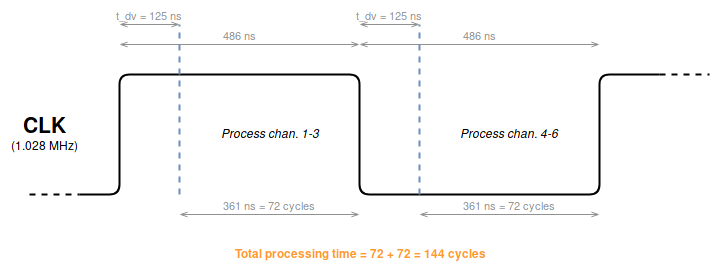
\includegraphics[width=1.0\linewidth]{Pictures/PRU_timing_diagram_mic_multiplexing.png}
\caption{Timing diagram of the processing times with mic multiplexing}
\label{fig:multiplex-mics}
\end{figure}

\begin{figure}[H]
\centering
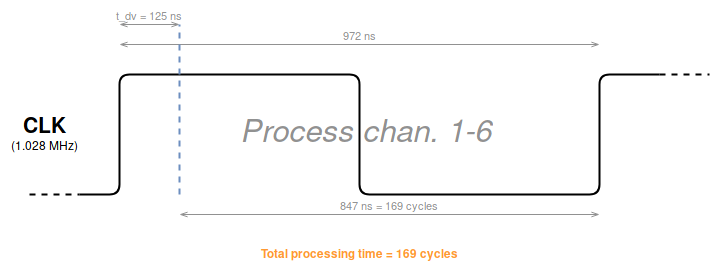
\includegraphics[width=1.0\linewidth]{Pictures/PRU_timing_diagram_no_mic_multiplexing.png}
\caption{Timing diagram of the processing times without mic
multiplexing}
\label{fig:nonmultiplex-mics}
\end{figure}

As mentioned above, multiplexing 2 microphones on 1 input pin reduces
the available processing time, as can be seen from Figures~\ref{fig:multiplex-mics} and ~\ref{fig:nonmultiplex-mics}.

\begin{figure}
\centering
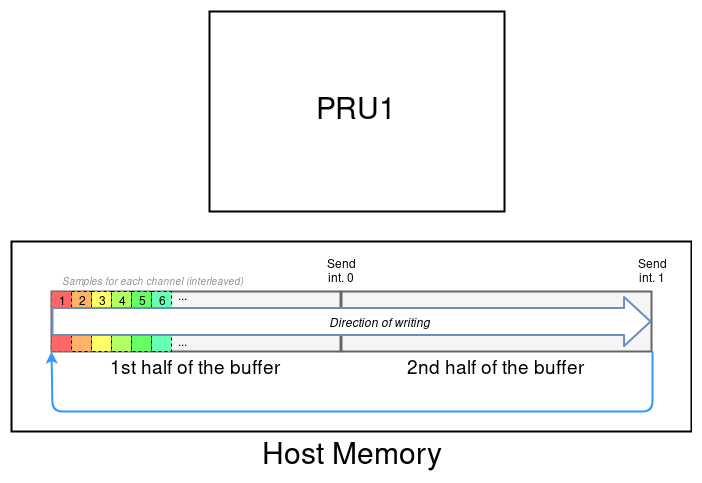
\includegraphics[width=0.8\linewidth]{Pictures/PRU_buffer.png}
\caption{Illustration of the interleaved samples in the buffer, and
interruptions}
\end{figure}

Reading the microphones' data is achieved by reading bits of the R31 register, which is connected to the PRU's input pins, to which the microphones' DATA lines are connected. Since we connected the microphones' clock to one of the input pins of the PRU as well, reading its state is done the same way. In order to know when to read the data, the PRU polls the CLK signal until it detects an edge. It then waits for 25 cycles (\texttt{t\_dv}) and finally reads the data and stores it in a register.

This register is the first integrator in the CIC filter and all subsequent integrators can be updated. Once this is done, the decimator is implemented by using a counter. The decimator uses that counter to determine whether it is time to update the comb stages or not. Once the comb stages are updated, some of the results of the CIC filter are ready and are written to the host's memory.

\hypertarget{usage-of-resources-depending-on-the-cic-filter-parameters-n-m-r-and-on-the-number-of-channels-c}{%
\subsection{\texorpdfstring{Usage of resources depending on the CIC
filter parameters and on the number of channels}{Usage of resources depending on the CIC filter parameters N, M, R and on the number of channels C}}\label{usage-of-resources-depending-on-the-cic-filter-parameters-n-m-r-and-on-the-number-of-channels-c}}

In the current design, we use only registers to store all values involved in the CIC filter computation. Each PRU has 32 registers \texttt{(r0-r31)}, but in practice only 30 are usable. This is because \texttt{r30} and \texttt{r31} are reserved for interacting with BBB GPIO pins and triggering interrupts.

Furthermore, since we use the PRU's 3 additional register banks, we cannot use all the bits of \texttt{r0}, because the value of the first byte of \texttt{r0} is used as an offset value for register exchanges with the banks.

Another thing we need to take into account is that, apart from channel private data (values involved in the CIC filter computations for each channel), we also need to keep track of some channel \textit{independent} data : a byte counter to keep track of the number of bytes written in the host buffer, a sample counter to implement decimation, the host buffer's size and address and temporary values used for delaying and processing input. This data has to stay on the PRU at all times.

We can fit the decimation counter in a single byte, as long as it does not exceed 255. However, the byte counter needs a complete register. The host's buffer size and address also each need one complete register. Finally, we can use one half register to store a temporary counter for implementing delays and also extracting single bits from the r31 register (input pins).

Also, in our implementation, even though we have 6 channels, we only have 3 output registers. After filling the 3 registers, their contents are written to the host buffer and they can be used to store new inputs.

We store all this information on PRU1 in the following way :

\begin{itemize}
\tightlist
\item
  \textbf{r0} : scratchpad offset (bits 0-7), decimation counter (bits
  8-15), delay counter / temporary storage for inputs (bits 16-31)
\item
  \textbf{r23, r24, r25} : temporary storage for outputs of the filter,
  could be only one register, but this would add more memory operations
  which would add overhead
\item
  \textbf{r26} : host buffer size
\item
  \textbf{r27} : host buffer physical address
\item
  \textbf{r28} : written bytes counter
\end{itemize}

The remaining registers are used for storing channel private data. In order to figure out how many registers we need for this, assuming one register is wide enough to hold the expected values (see Equation~\ref{eq:bout} above to check the required bit width), we can use the following formula \texttt{(M = 1)} :

\begin{verbatim}
n_reg_private = C * (N + 1 + N - 1 + N - 1) = C * (3N - 1)
\end{verbatim}

With \texttt{M\ !=\ 1}:

\begin{verbatim}
n_reg_private = C * (N + 1 + 2M * (N - 1))
\end{verbatim}

Where C is the number of channels, N and M are the parameters of the CIC
filter. It should be noted that \texttt{R} has no influence on the
filter's register usage. However, \texttt{R} influences the filter's
output data rate. In our case, \texttt{C\ =\ 6}, \texttt{M\ =\ 1},
\texttt{N\ =\ 4} and \texttt{R\ =\ 16}, so
\texttt{n\_reg\_private\ =\ 66}. This, along with the 7 registers holding channel independent data on
PRU1, gives us the total register usage :

\begin{verbatim}
n_reg_tot = C(3N - 1) + 7 = 66 + 7 = 73
\end{verbatim}

Note that different parameters may allow for fitting more than one
channel in a single register \footnote{if \texttt{B\textunderscore out} from Eq.~\ref{eq:bout} is $ \leq 16 $.}, which would change the above formula and
dramatically reduce the amount of registers needed.

We chose to keep \texttt{M = 1} because a greater value of \texttt{M} would increase the required number of registers by a significant amount. Furthermore, it is said in most documentation about CIC filters that keeping \texttt{M} to 1 or 2 suffices to provide a decent frequency response.


\hypertarget{total-number-of-registers-required-given-n-and-c-m-1-assuming-bit-width-of-32-is-enough}{%
\subsubsection{\texorpdfstring{Total number of registers required given
\texttt{N} and \texttt{C} (\texttt{M\ =\ 1}) (assuming bit width of 32
is
enough)}{Total number of registers required given N and C (M = 1) (assuming bit width of 32 is enough)}}\label{total-number-of-registers-required-given-n-and-c-m-1-assuming-bit-width-of-32-is-enough}}

\begin {table}[H]
\begin{center}
%	\scalebox{0.65}{%
\begin{tabular}{|c|c|c|c|c|c|c|}
	\hline  & \textbf{N} & \textbf{1} & \textbf{2} & \textbf{3} & \textbf{4} & \textbf{5} \\ 
	\hline \textbf{C} & & & & & & \\ 
	\hline  \textbf{1} & & 9 & 12 & 15 & 18 & 21 \\ 
	\hline \textbf{2} & & 11 & 17 & 23 & 29 & 35 \\ 
	\hline  \textbf{3} & & 13 & 22 & 31 & 40 & 49  \\ 
	\hline \textbf{6} & & 19 & 37 & 55 & 73 & 91 \\ 
	\hline \textbf{8} & & 23 & 47 & 71 & 95 & 119  \\ 
	\hline 
\end{tabular} 
\end{center}
\end {table}


An important thing to note is that the PRU is supposed to support the
\texttt{XCHG} instruction, which exchanges registers from the PRU to one of the
banks in one cycle. Unfortunately, it does not work. Only the \texttt{XIN} and
\texttt{XOUT} instructions currently work. This means that we always need to keep
\texttt{n\_reg\_private} (11) registers free to act as a temporary
storage place. The PRU's registers handle this task.

With the current parameters, storing all data on the PRU leaves one free
register : r29. Registers r1-r22 are used for channel private data and
are the ones exchanged with the scratchpads.

\subsubsection{Data rate of filter output}

We also want to figure out the data rate of the filter's output. To do
this, using the formula described earlier, we first compute the output
bit width \texttt{B\_out}. In our case, \texttt{B\_in\ =\ 1}, so
\texttt{B\_out\ =\ 17}. However, the PRU's registers are 32 bits wide
and it is more convenient to write the data in 32 bits chunks.
Therefore, our `effective' output bit width,
\texttt{B\_out'} is 32. Since we know the output sample
rate is \texttt{f\_s\ /\ R}, it is now straightforward to compute the
output data rate :

\begin{verbatim}
D_out = B_out * f_s / R
\end{verbatim}

\noindent Or using the \texttt{B\_out'} :

\begin{verbatim}
D_out' = B_out' * f_s / R
\end{verbatim}

\noindent In our case, \texttt{f\_s\ $ \approx $ 1.028\ MHz},
\texttt{R\ =\ 16} and \texttt{B\_out'\ =\ 32}, which
gives \texttt{D\_out'\ =\ 2.056\ Mb/s\ =\ 257~kB/s}.

\begin {table}[H]
\begin{center}
\begin{tabular}{|c|c|}
	\hline  & \textbf{\texttt{D\_out'\ (kB\ /\ s)}} \\ 
	\hline \textbf{R} &  \\ 
	\hline \textbf{16} & 257 \\ 
	\hline \textbf{32} & 128.5 \\ 
	\hline \textbf{48} & 85.7 \\ 
	\hline \textbf{64} & 64.3 \\ 
	\hline 
\end{tabular} 
\caption{Output data rate (kB / s) for 1 channel,
	given \texttt{R} (\texttt{M\ =\ 1},
	\texttt{B\_out'\ =\ 32}).}
\end{center}
\end{table}



\hypertarget{channel-proof-of-concept-program}{%
\subsubsection{1-channel ``proof of concept"
program}\label{channel-proof-of-concept-program}}

Before writing the 6-channels CIC filter and the C host interface, we wrote a simple, 1-channel, proof of concept program implementing a CIC filter. We then used this code as a base and adapted it for the 6-channels implementation. It can be found in \texttt{src/1Mic-CIC/} and run with \texttt{sh deploy.sh}. This will start recording from the microphone connected to P8.28 on the BeagleBone and then output the raw resulting PCM to a file in the \texttt{src/1Mic-CIC/output/} directory.

It follows the same basic principles as the 6-channels implementation, without scratchpad register exchanges, and waiting for only 1 channel instead of 6.

This implementation works and allowed us to have an idea of how the output of a channel sounds like with different parameters. The PCM signal can be converted to a wav file using the \texttt{PCMtoWAV.py} script in \texttt{wav\_conv/}.

\hypertarget{host-interface-and-api}{%
\section{Host interface and API}\label{host-interface-and-api}}

The host interface is written in C in the \texttt{interface.h} and
\texttt{interface.c} files. It is currently very simple and provides the
following functions :

\lstinputlisting{../src/6Mic-CIC/host/interface.h}


The host interface contains several components. The first is a special buffer in the host memory allocated by \texttt{prussdrv} which the PRU directly writes to. It contains the data computed by the PRU for all channels. The second component is a larger circular buffer which serves as the main temporary buffer of the interface.

When the \texttt{pru\_processing\_init()} function of the API is called, it loads and starts the PRU firmware and starts a separate thread which handles the recording of the samples from the PRU buffer to the bigger circular buffer of the interface. Everytime the PRU has finished writing one half of this buffer, it sends an interrupt to the host and starts writing to the other half. The code of the sent interrupt designates which half of the buffer was filled with fresh data.

This thread essentially waits alternatively for each interruption and then copies the corresponding buffer half to the circular buffer. Waiting for each interrupt alternatively makes sure the host cannot get desynchronized and start writing the buffer halves that are being overwritten by the PRU. However, this mechanism cannot detect whether a buffer half has been skipped. This can happen if the host is too busy with other programs which can make it miss an interrupt by the PRU. Furthermore, if an interrupt is missed, the next one will be skipped as well, since we wait for them alternatively. Therefore if an interrupt is missed, 2 buffer halves will actually be missed. We chose to use this mechanism because of its simplicity, and because it did not require the PRU to count the buffer halves it filled and output the number to the host regularly. This would however be a better solution.

The circular buffer is similar to a queue but with a fixed length. Its API provides functions for pushing and popping data from it. In the case of an overflow, the push function will only trigger a warning and overwrite the oldest data in the buffer.

The \texttt{pcm\_read} function provided by the API pops the number of samples required by the user from the circular buffer, then extracts only the number of channels the user asks for, and finally outputs this data to the user provided buffer.

It is important to note that there will be concurrent accesses to the circular buffer : data pushed by the recording thread, and data popped by the user thread calling the \texttt{pcm\_read} function. Our implementation handles this by making accesses mutually exclusive by using a mutex declared in the \texttt{interface.c} file. This is a simple but far from the ideal solution. For example, if a call to \texttt{pcm\_read} pops a large chunk of data from the circular buffer, this may block the recording for a long enough time that it will miss the next interrupt, and therefore a large chunk of samples.

\hypertarget{results}{%
\chapter{Results}\label{results}}

\hypertarget{single-channel-implementation}{%
\section{Single channel
implementation}\label{single-channel-implementation}}

The single channel implementation works and shows that it is possible to implement a CIC filter on the PRU and rely on PRU writes to the host memory. With the following parameters (N = 4, M = 1, R = 16), we were able to get a moderately noisy but intelligible signal at a sample rate of 64 kHz.

\begin{figure}[H]
\centering
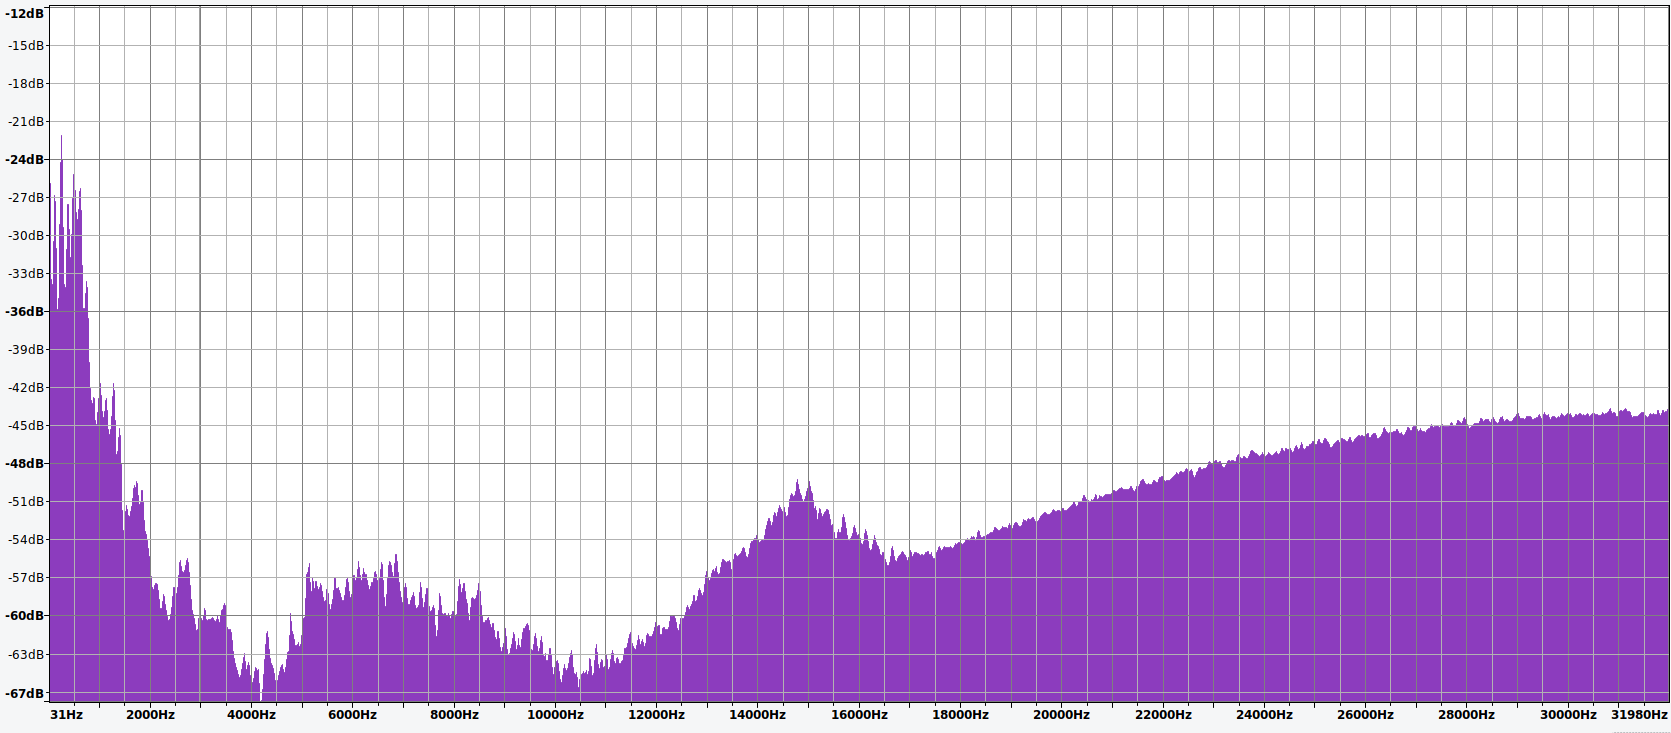
\includegraphics[width=0.8\linewidth]{Pictures/spectrogram.png}
\caption{Spectrogram of the signal of one of the channels from the demo recording made during the project's presentation.}
\end{figure}

It is worth noting that using one channel, the timing constraints are much less tight since there is much less processing to be done. This leaves more freedom in choosing the parameters. For example, higher input sample rates (compared to the 6-channel 1.028 MHz) are achievable.

\hypertarget{channels-implementation}{%
\section{6-channels implementation}\label{channels-implementation}}

At the time of writing this report, the 6-channels implementation works.

The C interface has been tested recording samples for up to 5 minutes and appears to work.

We have noticed that some occasional glitches appeared in the signal while using a microphone connected using a breadboard and soldered by hand. However, these glitches seem to have disappeared when we started using the Kurodako Board.

More rigorous testing needs to be done to make sure the PRU processing code and the interface work as intended.

\begin{figure}[H]
\centering
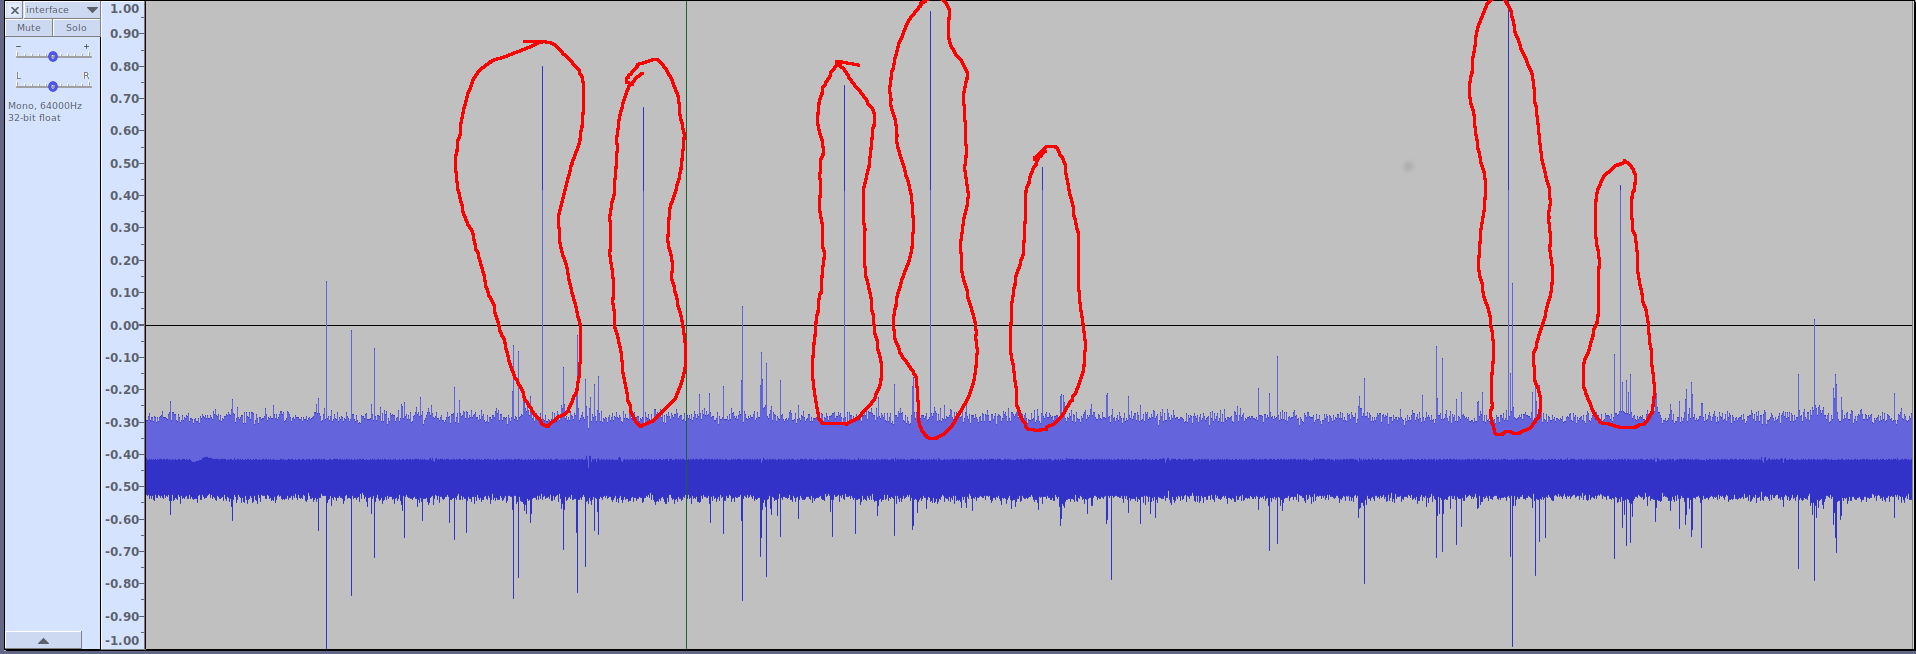
\includegraphics[width=0.8\linewidth]{Pictures/glitches_circled.png}
\caption{Glitches in the signal while recording for about 4m15s}
\end{figure}

\hypertarget{challenges-faced}{%
\chapter{Challenges faced}\label{challenges-faced}}

\hypertarget{lack-of-documentation-and-the-existence-of-2-different-drivers}{%
\section{Lack of documentation and the existence of 2, different
drivers}\label{lack-of-documentation-and-the-existence-of-2-different-drivers}}

The biggest challenge faced in this project is probably the lack of clear and organized documentation about how to run code on the PRU from the Linux host, how to configure the operating system so that the BeagleBone's pins can be multiplexed to the PRU, how to choose which driver to use, and finally how to configure the BeagleBone for it to work. Most of the documentation and examples are scarce, sometimes outdated and scattered across multiple websites which forced us to do a lot of trial and errors on things such as how to enable drivers or the right interrupts between the host and the PRU.

Apart from the fact that embedded systems is an inherently tough subject that is by far not as popular as higher level programming\footnote{in particular the PRU, which seems to be a piece of hardware very few people use or know about.}, I think the scarcity of the documentation is probably the greatest factor that makes the learning curve for this project rather steep.

\hypertarget{limited-number-of-registers-and-tight-timings}{%
\section{Limited number of registers and tight
timings}\label{limited-number-of-registers-and-tight-timings}}

On a more technical point of view, processing six channels simultaneously on one PRU is feasible, but challenging in terms of resource management. In our current implementation of the 6-channels CIC filter on the PRU, all operations required for processing one sample from each channel must execute in less than 144 cycles. All except one of the PRU's registers are used, and the majority of the banks' registers are used as well.

This `shortage' of registers on the PRU forced us to write each set of 6 samples in 2 steps of 3 registers and was the source of a bug : the byte offset counter used by the PRU to keep track of where it is writing in the host buffer was updated incorrectly. We incremented it by 6 * 4 bytes once instead of incrementing it by 3 * 4 bytes twice, which discarded the first 3 channels by overwriting them with the last 3 ones.

Another challenge was to design the program such that it would not rely on the host too much because of its unpredictable timings and busy nature. Below is an example of a bug that happened when the host was in charge of retrieving a new sample everytime it was ready (with these parameters, 64000 times per second). The host couldn't keep up and missed many samples, resulting in this quite weird looking (and sounding) spectrogram.

\begin{figure}[H]
\centering
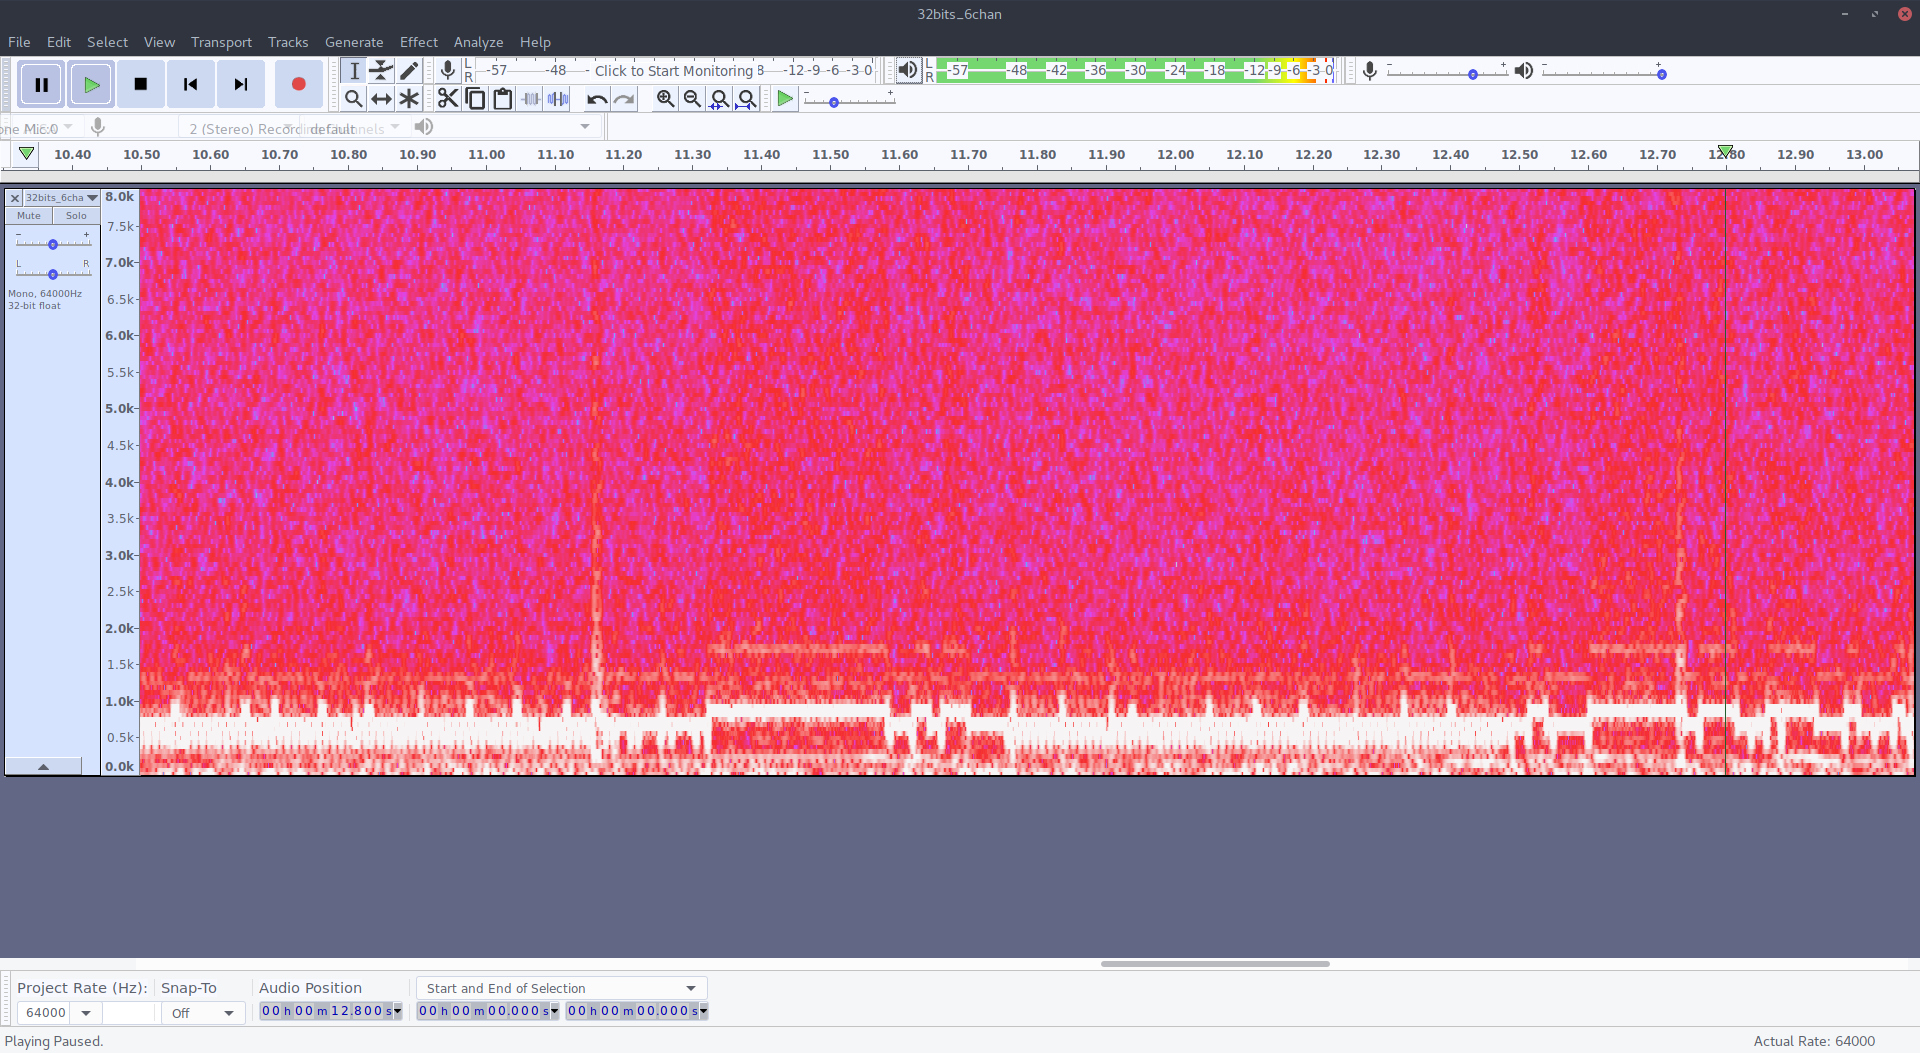
\includegraphics[width=1.0\linewidth]{Pictures/timing_bug.png}
\caption{Spectrogram of a signal missing samples as a result of timing
issues.}
\end{figure}

\hypertarget{possible-improvements-and-additional-features}{%
\chapter{Possible improvements and additional
features}\label{possible-improvements-and-additional-features}}

\hypertarget{use-both-prus}{%
\section{Use both PRUs}\label{use-both-prus}}

Currently, we use only one PRU (PRU1) to handle the audio processing with the CIC filter. The design choice was made to make the implementation simpler. However, this also limited us to being only able to process 6 channels at a time instead of the initial goal of 8.

It could for example be possible to implement a CIC on both PRUs which would allow us to handle more than 6 channels. Another idea would be to keep the CIC filter on one PRU, but move the compensation filter which is currently implemented on the host ARM CPU to the other PRU, offloading the ARM CPU even further and also reducing the latency.

\hypertarget{tweak-the-parameters-to-get-smaller-bit-width-and-possibly-handle-more-channels}{%
\section{Tweak the parameters to get smaller bit width and possibly
handle more
channels}\label{tweak-the-parameters-to-get-smaller-bit-width-and-possibly-handle-more-channels}}

The parameters we are currently using for the CIC filter (R = 16, N = 4, M = 1) give a decent frequency response (at least judging by our ear) but require 17 bits per stage of the filter. Tweaking the parameters to achieve 16 bits or less would allow fitting 2 channels in one register which would dramatically reduce the usage of memory resources, both on the PRU and on the host.


\hypertarget{use-of-a-lookup-table}{%
\section{Use of a lookup table}\label{use-of-a-lookup-table}}

Since the PRUs each have some data memory available (8 kB each, with an additional shared 12 kB), it might be more time-efficient to implement the PDM to PCM conversion using a precomputed look-up table stored in memory instead of implementing a CIC filter.

\hypertarget{better-and-more-modular-interface}{%
\section{Better and more modular
interface}\label{better-and-more-modular-interface}}

For now the interface is very limited, and depending on how many channels the user chooses to read, the whole program can also be very wasteful on resources. This is because with the current implementation, the PRU always processes the 6 channels, and the host interface's backend always records all 6 channels, even if in the end the user requests fewer channels. In the event the user wants to read fewer channels, the interface's front-end will just drop the data from the channels the user does not want, before sending the data to the user.

An improvement could be to let the user choose how many channels he intends to use at most, and then only handle this number of channels instead of the maximum possible. However, making the CIC filter's code modular might not be a feasible task given the high performance requirements, at least with the current model of our implementation. A workaround would be to write several programs, possibly one for each number of channels, and load the appropriate one on the PRU by letting the user choose the number of channels when calling the \texttt{pru\_processing\_init} function is called.

As explained earlier, the current implementation of the interface uses a very simple circular buffer we implemented ourselves, and concurrent accesses are managed using a mutex. This is probably a quite inefficient and unoptimized solution that could lead the interface back-end to miss the recovery of some of the samples from the PRU, if the \texttt{pcm\_read} function is asked to retrieve a huge chunk of data.

A workaround to this would be to implement a 'smarter' concurrent circular buffer, or use of an existing one. One solution we considered but eventually did not have enough time to use was the \texttt{liblfds}\footnote{\url{https://liblfds.org/}} library, which contains an implementation of a thread-safe, concurrent cirular buffer (ringbuffer).

Another idea would be to adapt the interface so that it could directly create a WAV file, and not a raw PCM file.

\hypertarget{introduce-further-filtering-on-the-host-side}{%
\subsection{Introduce further filtering on the host
side}\label{introduce-further-filtering-on-the-host-side}}

As mentioned before, CIC filters are very efficient filters but they lack a flat frequency response with a sharp cutoff and we need an additional compensation filter appended after them to get a better response. The current implementation of the host interface does not implement such a filter yet but this is a possible and probably very useful improvement that could be made. A nice feature to have could be to make it modular such that it can accept many different types of compensation filters.

\hypertarget{acknowledgments}{%
\chapter{Acknowledgments}\label{acknowledgments}}

I would like to offer my special thanks to Eric Bezzam for his continuous assistance throughout the semester. He provided me with valuable explanations about some of the signal processing theory and nomenclature, which made understanding the motivation and goals of the project easier for me. He also greatly helped me by writing some useful little programs for converting PCM signals to WAV, plotting the filter's power response, and analizing timings in the PRU.

I would also like to thank Robin Scheibler, my supervisor for this project, for his valuable pieces of advice he gave throughout the project.

I would like to also thank the people who were there at the midterm presentation for their valuable remarks and advices, such as the idea of using a look-up table for the filter.

\hypertarget{sources-and-bibliography}{%
\chapter*{Sources and bibliography}\label{sources-and-bibliography}}

\begin{itemize}
\tightlist
\item
  CIC Filter theory :
  
  

  \begin{itemize}
  \tightlist
  \item
    Hogenauer, Eugene. \emph{"An Economical Class of Digital Filters
    For Decimation and Interpolation"} \url{https://www.researchgate.net/publication/3176890_An_economical_class_of_digital_filters_for_decimation_and_interpolation}
  \item
    \url{https://en.wikipedia.org/wiki/Cascaded_integrator%E2%80%93comb_filter}
  \item
    \url{https://dspguru.com/files/cic.pdf}
  \item
    \url{https://www.embedded.com/design/configurable-systems/4006446/Understanding-cascaded-integrator-comb-filters}
  \end{itemize}
\item
  PRU programming :

  \begin{itemize}
  \tightlist
  \item
    \url{http://processors.wiki.ti.com/index.php/PRU\_Assembly\_Instructions}
  \item
    \url{http://www.embedded-things.com/bbb/understanding-bbb-pru-shared-memory-access/}
  \item
    \url{http://credentiality2.blogspot.ch/2015/09/beaglebone-pru-gpio-example.html}
  \item
    \url{https://theembeddedkitchen.net/tag/beaglebone}
  \item
    \url{http://www.ti.com/lit/wp/spry264a/spry264a.pdf}
  \item
    \url{http://processors.wiki.ti.com/index.php/PRU\_Linux\_Application\_Loader\_API\_Guide}
  \end{itemize}
\item
  Host configuration :

  \begin{itemize}
  \tightlist
  \item
    \url{http://catch22.eu/beaglebone/beaglebone-pru-uio/}
  \item
    \url{https://www.teachmemicro.com/beaglebone-black-pwm-ubuntu-device-tree/}
  \item
    \url{http://www.dangtrinh.com/2015/05/sharing-internet-with-beaglebone-black.html}
  \item
    \url{https://beagleboard.org/getting-started}
  \end{itemize}
\end{itemize}
\end{document}
